\documentclass{article}
\usepackage[letterpaper,margin=1in]{geometry}
\usepackage{xcolor}
\usepackage{fancyhdr}
\usepackage{tgschola} % or any other font package you like
\usepackage{setspace}
\usepackage{graphicx}

\pagestyle{fancy}
\fancyhf{}
\fancyhead[C]{%
  \footnotesize
  Avi Vajpeyi  \hspace{35pt}
 CS 200 - Junior Independant Study \hspace{35pt}
 \today }

\newcommand{\soptitle}{Software Description}
\newcommand{\yourname}{Avi Vajpeyi}
\newcommand{\youremail}{avajpeyi18@wooster.edu}
\newcommand{\yourweb}{}

\newcommand{\statement}[1]{\par\medskip
  \underline{\textcolor{blue}{\textbf{#1:}}}\space
}

\usepackage[
  colorlinks,
  breaklinks,
  pdftitle={\yourname - \soptitle},
  pdfauthor={\yourname},
  unicode
]{hyperref}

\begin{document}

\begin{center}\LARGE\soptitle\\
\large for Chaotic Scattering for a Sliding Mass in a Complex Topography
\end{center}

\hrule
\vspace{1pt}
\hrule height 1pt

\bigskip


{\setstretch{1.5} 
	
	
	\fontfamily{ptm}\selectfont
	\normalsize{
	This project relies on using  numerical integration algorithms such as Euler-Cromer, and the adaptive four stage Runge-Kutta, to calculate the trajectory of a particle entering a region with four hills. Depending on the initial $y$ position of the particle, the particle exits the region at a particular angle with respect to the $x$ axis. The behavior of the particle`s initial position to the exit angle is analysed. 
	
	
	\begin{figure}[h]
		\centering
		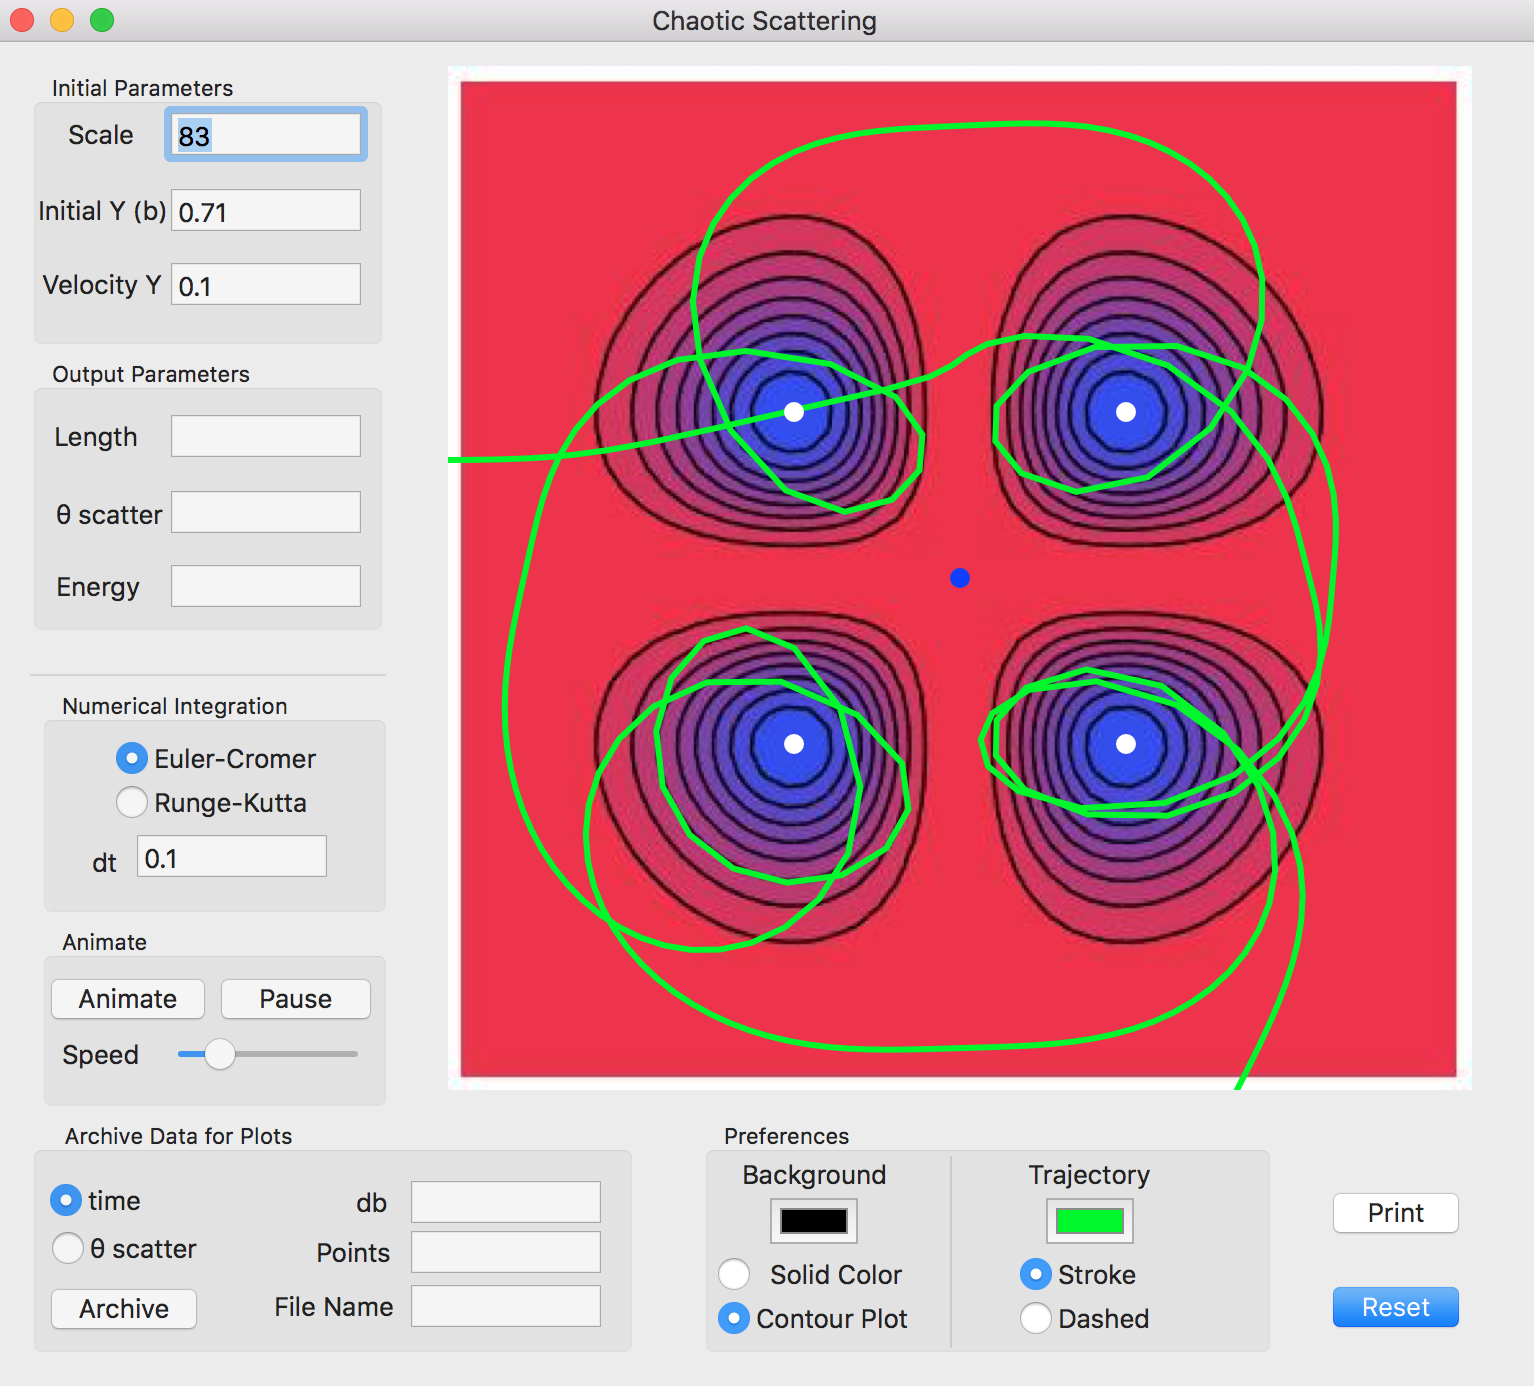
\includegraphics[width=0.8\textwidth]{image1.png}
		\caption{A screen shot of the application. The blue lines represent the potentials of the system while the green line traces the path of the particle. }
		\label{fig:chaos}
	\end{figure}
	
	
	
	We implement this model in a Coca application for the OS X. The program is in Objective C, and we rely on the various tools available via the Coca API to run it. Xcode is the IDE we use to construct the simulation, as it provides a straightforward method of creating the interface for the application. 
 
	The application consists of a window with a view of a two-dimensional plane, displaying the four hills, and the particle at a distance from the hills, as seen in figure~\ref{fig:chaos}. The trajectory of the particle, can be adjusted by changing the initial position along the $y$ axis. Alternately, the starting position of the particle can be set within the `Initial Y (b)' text field. The `b' is the symbol for the impact parameter used in comparable simulations for chaotic scattering. The particle's velocity, another inpt parameter can be changed within the text field marked `Velocity Y'. Initially, the potential hills are present in the coordinates $(\pm 1, \pm 1)$. The scale input parameter shifts the centers of the hills outwards, and makes the hills bigger. Hence, it allows the user to enlarge the transit of the particle. This will later be implemented in the form of a magnifying glass that the user can use to zoom into a region of the particle's path.
	
	Once these input values are provided, the simulation can either generate a path as shown in the figures, or display an animation of a particle traversing the potentials with the `Animate' button. Additionally before plotting the trajectory, there is an option of using switching between the Euler-Cromer algorithm, and the four stage Runge-Kutta algorithm. Thereby, users can observe how the two numerical integration techniques alter the path of the particle. 
	
	After the particle finishes its transit, it exits the system at a specific time, and angle from the x axis. The `Archive' button runs the simulation for a set of initial Y positions and records the various exit times and angles of the particle from the  system. This data when plotted displays interesting fractal patterns which we can print with the simulation and analyse.\\
	
	
	The most challenging portion of this program is determining the potentials of the four hills, and making the particle follow the potentials near the hills. Additionally, making the animation to push a particle forward through the path was an intricate problem. However, the fact that this simulation provides new insights to the chaotic scattering problem makes the investigation worth while. 
	
	
	}






\begin{figure}[h]
	\centering
	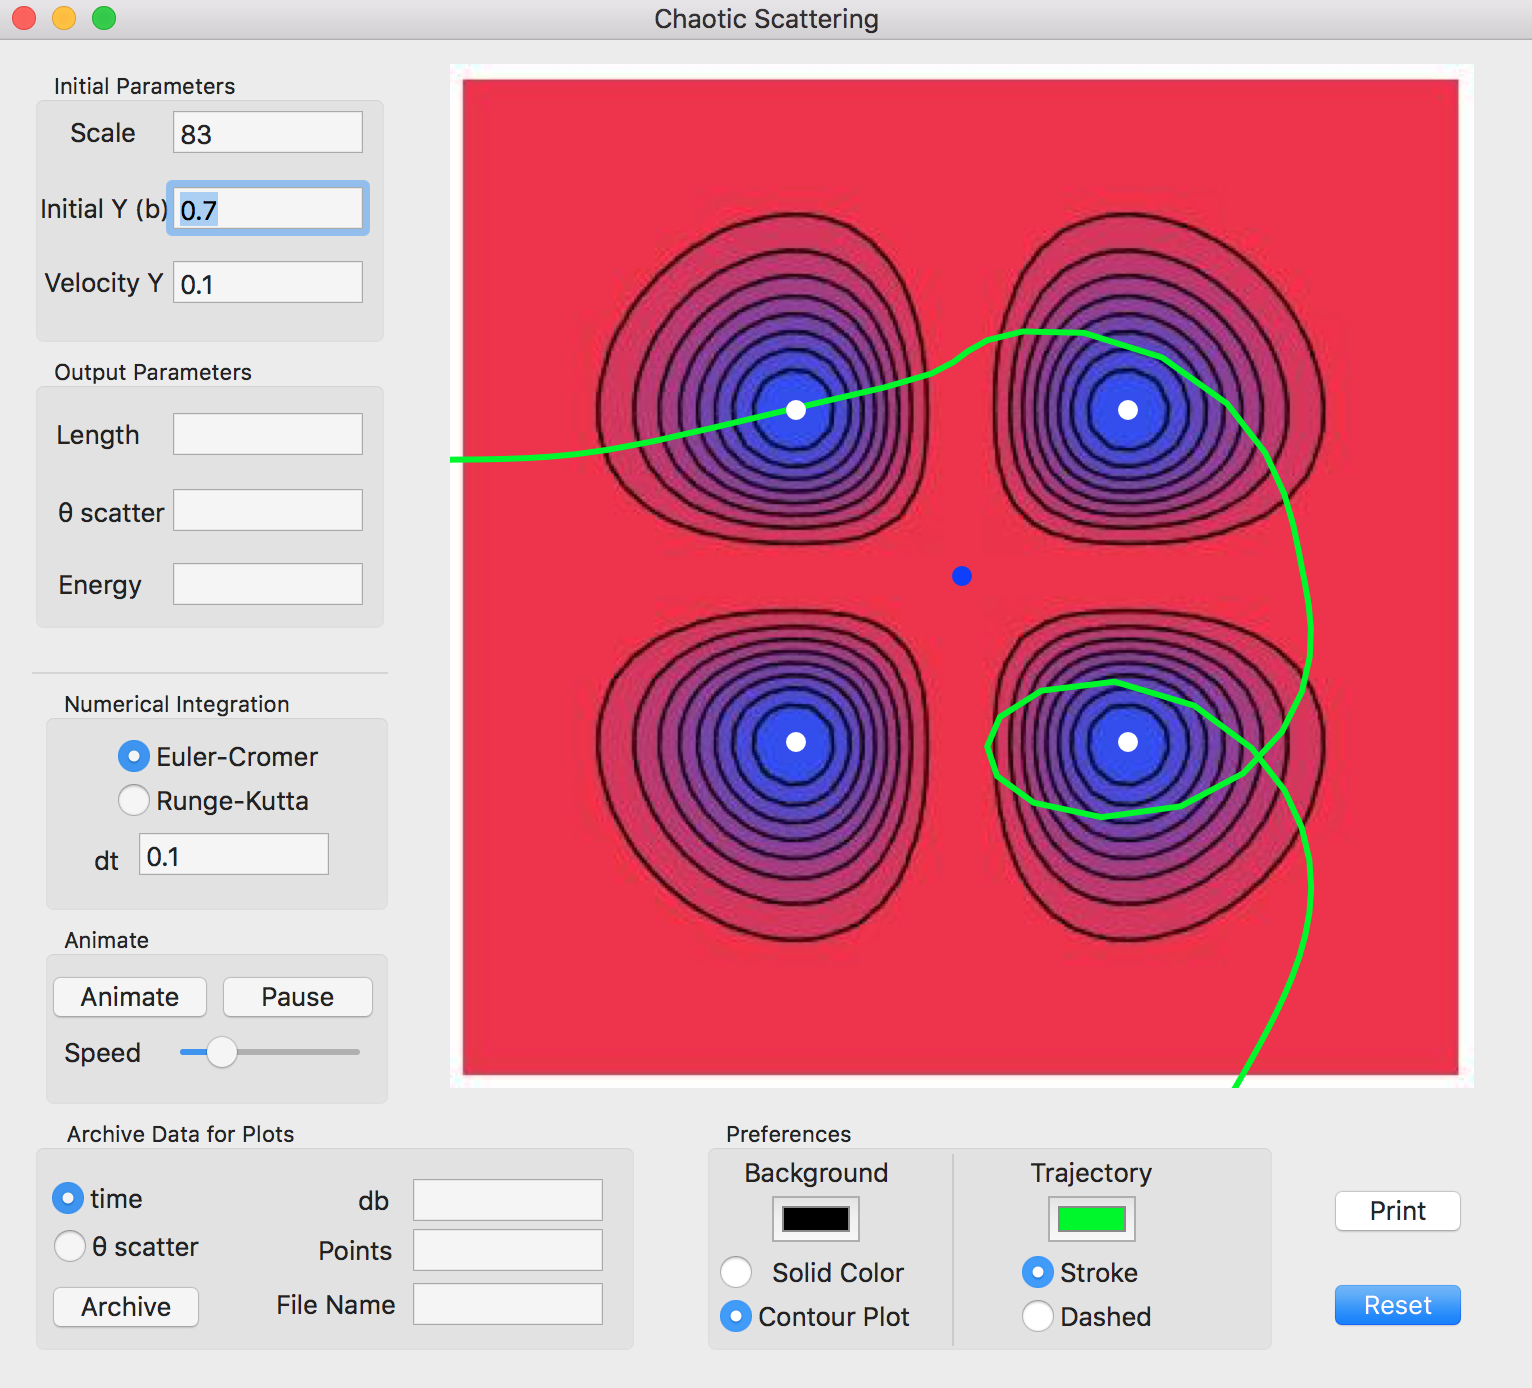
\includegraphics[width=0.7\textwidth]{image2.png}
	\caption{A similar screen as in Fig~1, however with its initial y position altered by a factor of 0.01. This clearly differs by a great amount from the first one, displaying the chaotic nature of the system. }
	\label{fig:chaos2}
\end{figure}








}


 

\end{document}